% zhoukan_content.tex - 周练卷题目内容（由程序自动生成，勿手动修改）
% 此文件被 student / teacher / onepage 三个 wrapper 共享 \input
% ============================================================
% 可配置变量（调用时由外部替换 {{{var}}}} 占位符）
% 使用 \providecommand 允许 wrapper 先定义再覆盖
% ============================================================
\providecommand{\weekNumber}{}           % 第X周，如 "第5周"，为空则不显示
\providecommand{\zhoukanDate}{日期}
\providecommand{\zhoukanClass}{班级}
\providecommand{\zhoukanStudent}{姓名}
\providecommand{\zhoukanMode}{limited}   % limited=限时训练(30-45min) | homework=巩固作业(不限时)
\providecommand{\suggestedTime}{45分钟}  % 建议用时
\providecommand{\weekFocus}{本周重点知识点} % 可多行，用 \\ 换行
% 题量控制（用户必须指定，无默认值）
\providecommand{\mcqCount}{4}
\providecommand{\msqCount}{1}
\providecommand{\blankCount}{2}
\providecommand{\saqCount}{1}
% 题型间距控制
\providecommand{\mcqItemSep}{0.3em}
\providecommand{\msqItemSep}{0.5em}
\providecommand{\blankItemSep}{0.8em}
\providecommand{\saqItemSep}{2.5cm}
% 选择题选项列数
\providecommand{\mcqTasksCols}{4}
\providecommand{\msqTasksCols}{2}
% ============================================================

%===== 题目内容开始 =====%

% ── 周练信息栏 ──
\begin{center}
    \LARGE\textbf{数学周练}
    \ifx\weekNumber\empty\else\ \weekNumber\fi
\end{center}
\vspace{0.5em}

\noindent\begin{tabular}{@{}p{0.25\textwidth}p{0.25\textwidth}p{0.25\textwidth}p{0.25\textwidth}@{}}
    \textbf{日期：}\zhoukanDate & \textbf{建议用时：}\suggestedTime & \textbf{班级：}\zhoukanClass & \textbf{姓名：}\zhoukanStudent \\
\end{tabular}

\ifx\weekFocus\empty\else
\vspace{0.5em}
\noindent\textbf{本周重点：}\par\weekFocus
\fi

\vspace{1em}
\hrule
\vspace{1em}

% ============================================================
% 四大题固定结构（题量由变量控制）
% ============================================================

% ── 一、选择题（单选）──
\noindent\textbf{一、选择题（单选，共 \mcqCount\ 小题，每小题 5 分）}
\vspace{0.3em}
\begin{enumerate}[itemsep=\mcqItemSep]
    % 题量由生成脚本根据 \mcqCount 生成对应数量的 \item
    % 此处为示例，展示 4 题
    \item 已知集合 $A=\{x \mid x^2-3x+2=0\}$，$B=\{0,1,2\}$，则 $A \cup B =$
    \begin{tasks}(\mcqTasksCols)
        \task $\{0\}$
        \task $\{0,1,2\}$
        \task $\{1,2\}$
        \task $\{0,1\}$
    \end{tasks}
    \begin{solution}
        \daan{B}
        \jieti 解方程得 $A=\{1,2\}$，故 $A\cup B=\{0,1,2\}$。
        \xijie 基础集合运算，解一元二次方程求集合后直接并集。
        \cuowu 易将 $A$ 解为 $\{2,3\}$ 或 $\{0,1\}$，注意 $x^2-3x+2=0$ 根为 $1,2$。
        \pingfen 选对得 5 分，选错得 0 分。
    \end{solution}

    \item 若复数 $z$ 满足 $z(1+\mathrm{i})=2\mathrm{i}$，则 $z$ 的共轭复数为
    \begin{tasks}(\mcqTasksCols)
        \task $1+\mathrm{i}$
        \task $1-\mathrm{i}$
        \task $-1+\mathrm{i}$
        \task $-1-\mathrm{i}$
    \end{tasks}
    \begin{solution}
        \daan{B}
        \jieti $z=\frac{2\mathrm{i}}{1+\mathrm{i}}=\frac{2\mathrm{i}(1-\mathrm{i})}{2}=1+\mathrm{i}$，共轭为 $1-\mathrm{i}$。
        \xijie 复数除法有理化分母。
        \pingfen 选对得 5 分。
    \end{solution}

    \item 已知向量 $\vec{a}=(1,2)$，$\vec{b}=(3,4)$，则 $|\vec{a}+\vec{b}|=$
    \begin{tasks}(\mcqTasksCols)
        \task $2\sqrt{5}$
        \task $2\sqrt{10}$
        \task $10$
        \task $20$
    \end{tasks}
    \begin{solution}
        \daan{B}
        \jieti $\vec{a}+\vec{b}=(4,6)$，$|\vec{a}+\vec{b}|=\sqrt{16+36}=\sqrt{52}=2\sqrt{13}$。
        \pingfen 选对得 5 分。
    \end{solution}

    \item 设函数 $f(x)=x^3-3x^2+2$，则 $f(x)$ 在区间 $[-1,3]$ 的最小值为
    \begin{tasks}(\mcqTasksCols)
        \task $-2$
        \task $0$
        \task $2$
        \task $4$
    \end{tasks}
    \begin{solution}
        \daan{A}
        \jieti $f'(x)=3x^2-6x=3x(x-2)$，驻点 $x=0,2$，端点 $x=-1,3$，比较 $f(-1)=-2, f(0)=2, f(2)=-2, f(3)=2$，最小值为 $-2$。
        \xijie 导数求闭区间最值，核心是求驻点并比较端点函数值。
        \cuowu 易漏算端点 $x=-1$ 的函数值，或驻点判断错误。
        \pingfen 选对得 5 分。
    \end{solution}
\end{enumerate}

% ── 二、选择题（多选）──
\ifnum\msqCount>0
\vspace{1em}
\noindent\textbf{二、选择题（多选，共 \msqCount\ 小题，每小题 6 分）}
\vspace{0.3em}
\begin{enumerate}[start=\numexpr\mcqCount+1, itemsep=\msqItemSep]
    \item 设 $z = 3 + 2\mathrm{i}$，则
    \begin{tasks}(\msqTasksCols)
        \task $\bar{z} = 3 - 2\mathrm{i}$
        \task $|z| = \sqrt{13}$
        \task $z^2 = 5 + 12\mathrm{i}$
        \task $\dfrac{z+3}{z-\mathrm{i}} \in \mathbb{R}$
    \end{tasks}
    \begin{solution}
        \daan{ABD}
        \jieti $\bar{z}=3-2\mathrm{i}$，$|z|=\sqrt{13}$，$z^2=5+12\mathrm{i}$，$\frac{z+3}{z-\mathrm{i}}\in\mathbb{R}$。
        \xijie 复数四则运算、模、共轭、实数判断综合考查。
        \pingfen 全对得 6 分，选对少选得 3 分，有选错得 0 分。
    \end{solution}
\end{enumerate}
\fi

% ── 三、填空题 ──
\ifnum\blankCount>0
\vspace{1em}
\noindent\textbf{三、填空题（共 \blankCount\ 小题，每小题 5 分）}
\vspace{0.3em}
\begin{enumerate}[start=\numexpr\mcqCount+\msqCount+1, itemsep=\blankItemSep]
    \item 若直线 $y=2x+5$ 是曲线 $y=\mathrm{e}^x+x+a$ 的一条切线，则 $a=$ \blank.
    \begin{solution}
        \daan{$4-\ln 2$}
        \jieti 设切点 $(x_0,y_0)$，导数 $\mathrm{e}^{x_0}+1=2\Rightarrow x_0=0$，代入得 $a=4-\ln 2$。
        \pingfen 答案正确得 5 分，过程有误扣分。
    \end{solution}

    \item 已知双曲线 $C$ 的虚轴长是实轴长的 $\sqrt{7}$ 倍，则 $C$ 的离心率为 \blank.
    \begin{solution}
        \daan{$2\sqrt{2}$}
        \jieti $b=\sqrt{7}a$，$c=\sqrt{a^2+b^2}=2\sqrt{2}a$，$e=2\sqrt{2}$。
        \pingfen 答案正确得 5 分。
    \end{solution}

    \item 函数 $f(x)=\sin x + \cos x$ 在 $[0,\pi]$ 的最大值为 \blank.
    \begin{solution}
        \daan{$\sqrt{2}$}
        \jieti $f(x)=\sqrt{2}\sin(x+\frac{\pi}{4})$，在 $[0,\pi]$ 内最大值为 $\sqrt{2}$。
        \pingfen 答案正确得 5 分。
    \end{solution}
\end{enumerate}
\fi

% ── 四、解答题 ──
\ifnum\saqCount>0
\vspace{1em}
\noindent\textbf{四、解答题（共 \saqCount\ 小题，分值标注）}
\vspace{0.3em}
\begin{examenum}[itemsep=\saqItemSep]

    \item （12分）已知数列 $\{a_n\}$ 中，$a_1=3$，$\dfrac{a_{n+1}}{n}=\dfrac{a_n}{n+1}+\dfrac{1}{n(n+1)}$.
    \begin{examenum}
        \item 证明：数列 $\{na_n\}$ 是等差数列；
        \item 给定正整数 $m$，设函数 $f(x)=a_1x+a_2x^2+\cdots+a_mx^m$，求 $f'(-2)$.
    \end{examenum}
    \begin{solution}
        \daan{(1) 略 (2) $f'(-2)=3\cdot 2^{m-1}(m-2)+(-2)^m$}
        \jieti (1) 由递推式得 $(n+1)a_{n+1}-na_n=1$，故 $\{na_n\}$ 公差 1 的等差数列。\par (2) $na_n=3n\Rightarrow a_n=3$，$f(x)=3\sum_{k=1}^m x^k$，求导代入 $x=-2$。
        \xijie 构造 $na_n$ 化为等差数列，求通项后求多项式导数。
        \cuowu 易漏掉 $a_n$ 推导，直接求和出错；导数代入符号错误。
        \pingfen (1) 证明过程完整得 6 分，关键步骤缺失扣分；(2) 结果正确得 6 分，过程分 3 分。
        \zongjie 本周核心：数列递推构造等差/等比、多项式求导、闭区间最值、复数运算。下周预习：圆锥曲线定义与标准方程。
    \end{solution}

    \item （15分）如图，在四棱锥 $P-ABCD$ 中，$PA\perp \text{底面}\ ABCD$，$AB\perp AD$，$BC\Parallel AD$。
    \begin{examenum}
        \item 证明：$\text{平面}\ PAB\perp \text{平面}\ PAD$；
        \item 设 $PA=AB=\sqrt{2}$，$BC=2$，$AD=1+\sqrt{3}$，且点 $P,B,C,D$ 均在球 $O$ 的球面上。
        \begin{examenum}
            \item 证明：点 $O$ 在平面 $ABCD$ 内；
            \item 求直线 $AC$ 与 $PO$ 所成角的余弦值。
        \end{examenum}
    \end{examenum}
    \begin{solution}
        \daan{(1) 略 (2)(i) 略 (ii) $\frac{\sqrt{6}}{3}$}
        \jieti (1) $AB\perp AD$ 且 $PA\perp ABCD\Rightarrow AB\perp$ 平面 $PAD$，$AB\subset PAB$，两平面垂直。\par (2) 建立坐标系 $A(0,0,0), B(\sqrt{2},0,0), D(0,1+\sqrt{3},0), C(2,1+\sqrt{3},0), P(0,0,\sqrt{2})$，球心 $O$ 到四点等距解得坐标，向量法求角。
        \xijie 立体几何证明+球几何+向量夹角，综合性强。
        \cuowu 坐标系建立不当；球心位置判断忽略投影条件；向量模长计算失误。
        \pingfen (1) 6 分；(2)(i) 4 分；(ii) 5 分，步骤分各 2-3 分。
    \end{solution}

\end{examenum}
\fi

% ── 图示占位 ──
\vspace{1em}
\begin{center}
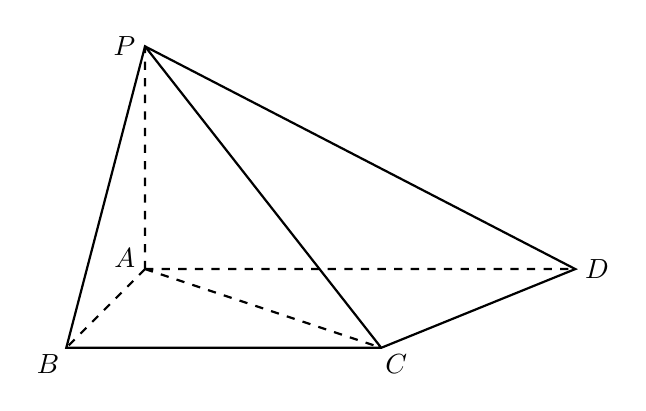
\begin{tikzpicture}
    \coordinate (A) at (0,0);
    \coordinate (B) at (-1,-1);
    \coordinate (C) at (3,-1);
    \coordinate (D) at ({2+2*sqrt(3)},0);
    \coordinate (P) at (0,{2*sqrt(2)});
    \node[above left,yshift=-3] at (A) {$A$};
    \node[right] at (D) {$D$};
    \node[left] at (P) {$P$};
    \node[below left,xshift=1,yshift=1] at (B) {$B$};
    \node[below right,xshift=-2,yshift=1] at (C) {$C$};
    \draw[dashed,thick] (A) -- (B) (A) -- (C) (A) -- (D) (A) -- (P);
    \draw[thick] (P) -- (B) -- (C) --(D) -- cycle (P) -- (C);
\end{tikzpicture}
\captionof{figure}{\textbf{图1：四棱锥 $P-ABCD$ 示意图}}
\end{center}

%===== 题目内容结束 =====%